% !TEX root = FDS_Technical_Reference_Guide.tex

\typeout{new file: HVAC_Chapter.tex}

\chapter{Heating, Ventilation, and Air Conditioning (HVAC)}

HVAC systems are found throughout the built environment.  During a fire, HVAC ducts can serve as a path for heat and combustion products to be moved through a building, and the ducts can serve as a supply of fresh air for the fire.  In some facilities, such as data centers and clean rooms, fire detection devices are placed inside of HVAC ducts. HVAC systems may also serve as part of the fire protection system for a building when used to exhaust smoke or maintain stairwell pressurization.

While simple defined velocity, mass flux, or pressure boundary conditions can represent inflow and outflow due to HVAC system, they cannot fully model an HVAC system. There is no coupling of the mass, momentum, and energy solutions amongst the multiple inlets and outlets comprising the HVAC network. To address this limitation, an HVAC network solver has been added to FDS.

The reader may find it useful to read a literature review on coupled hybrid modeling in fire applications~\cite{Ralph:1} and review similar work in coupling CFD to a 1-D nodal model for analysis of ventilation in tunnel fires \cite{Colella:2010, Colella:2011}.

\section{Governing Equations}

The overall HVAC solver is based on the MELCOR~\cite{MELCOR} thermal hydraulic solver.  MELCOR is a computer program for simulating accidents in nuclear power plant containment buildings.
The Fire and Smoke Simulator (FSSIM)~\cite{FSSIM}, a network fire model, has shown prior success in using the MELCOR solver to model fire spread and smoke movement
in the presence of complex ventilation systems, and the FDS implementation of the MELCOR solver is largely based on the implementation found in FSSIM.  The coupling of the HVAC solver to the remainder of the FDS computation is in part based upon approaches taken in GOTHIC~\cite{GOTHIC}, another containment analysis code that couples CFD-like features for large containment volumes with a network model for piping and ventilation.

The MELCOR solver uses an explicit solver for the conservation equations of mass and energy combined with an implicit solver for the conservation of momentum equation. An HVAC system is represented as a network of nodes and ducts.  A node represents where a duct joins with the FDS computational domain or where multiple ducts are joined such as at a tee joint. A duct segment in the network represents any continuous flow path not interrupted by a node, and as such may include multiple fittings (elbows, expansions, or contractions, etc.)
and may have varying area over its length. The nodal conservation equations of
mass, energy, and momentum (in that order) are:
\be \sum\limits_{j} \rho_j \, u_j \, A_j = 0   \label{HVACmass} \ee
\be \sum\limits_{j} \rho_j \, u_j \, A_j \, h_j= 0   \label{HVACenergy} \ee
\be \rho_j L_j \frac{\d u_j}{\d t} = \left(p_i - p_k\right)+\left(\rho g \Delta z\right)_j+\Delta p_j - \frac{1}{2}K_j \rho_j \left| u_j \right| u_j  \label{HVACmomentum} \ee
where $u$ is the duct velocity, $A$ is the duct area, and $h$ is the enthalpy of the fluid in the duct.
The subscript $j$ indicates a duct segment, the subscripts $i$ and $k$ indicate nodes (where one or more ducts join or where a duct terminates in a compartment).
$\Delta p$ is a fixed source of momentum (a fan or blower), $L$ is the length of the duct segment, and $K$ is the total dimensionless loss coefficient of the duct segment (which includes wall friction losses and minor losses).

Since nodes have no volume, the mass and energy conservation equations require that what flows into a node must also flow out. In the momentum equation the terms on the right hand side consist of the pressure gradient between the upstream and the downstream node, the buoyancy head, pressure rise due to an external source (e.g., a fan or blower), and the pressure losses due to wall friction or the presence of duct fittings. In its default mode of operation, the transport delay of mass and energy along the length of a duct is not accounted for. An optional model for this delay is available and described in Sec.~\ref{sec:duct_transport}.

\section{Solution Procedure}

The momentum equation (\ref{HVACmomentum}) is non-linear with respect to velocity due to
the loss term.  Additionally, the pressure difference between two nodes in the network is impacted by the pressure change at all
nodes coupled to that duct either directly (part of the same duct network) or indirectly (connected to the same compartment as another duct network).
Solving the momentum equation, requires accounting for both of these.  This is done with the following discretization:
\be u^{n+1}_j=u^{n}_j + \frac{\Delta t^n}{\rho_j L_j} \left[ \left(\tilde{p}^n_i - \tilde{p}^n_k\right)+\left(\rho g \Delta z\right)^{n}_j+\Delta p^{n}_j -
   \frac{1}{2}K_j \rho_j \left(\left|u^{n-}_j+u^{n+}_j\right|u^{n+1}_j-\left|u^{n+}_j \right|u^{n-}_j \right) \right] \label{HVACdiscretemomentum} \ee
The superscripts $n+$ and $n-$ on the velocity are used to linearize the flow loss in a duct to avoid a non-linear differential equation for velocity.
The $n+$ superscript is the prior iteration value and the $n-$ is either the prior iteration value or zero if flow reversal occurred between iterations.
This approach is used to speed convergence when duct flows are near zero to avoid large changes in $K$ if the forward and reverse losses are markedly different.
Note that the node pressures are not expressed as $P^n_i$, but rather as $\tilde{p}^n_i$.  This indicates an extrapolated pressure at the end of the current time step
rather than the actual pressure at the end of the time step.  The pressure in a compartment is a function of the mass and energy flowing in and out.
If that compartment is connected to other compartments by doors or other openings, then the pressure is also dependent upon flows into and out those other compartments.
Those mass and energy flows include both those being predicted by the HVAC model and those being predicted by the CFD model.
For example, in Fig.~\ref{hvacpressure}, the un-shaded compartments have pressure solutions that are dependent upon the flows predicted by both the
HVAC model and the CFD model and all of those compartments need to be included in the extrapolated pressure for those compartments.
Since the two models are not fully coupled, the extrapolated pressure is an estimate of the pressure at the end of the time step based upon the pressure rise for the prior time step.

\begin{figure}[ht!]
   \begin{center}
      \scalebox{0.8}{\includegraphics{FIGURES/hvacpressure}}
      \caption[Illustration of interdependent pressure solutions]{\label{hvacpressure} Illustration of interdependent pressure solutions.  All un-shaded compartments have pressures that are dependent upon each other.}
   \end{center}
\end{figure}

The extrapolated pressure for a compartment can be determined by using Eq.~(\ref{concon2}) and correcting the integral over velocity for the current solution of
all interdependent HVAC flows into or out of an FDS pressure zone:
\be \tilde{p}^n_i  = p^{n-1}_i+\left(\frac{\d p^{n-1}_i}{\d t} + \frac{{\sum_j u^{n}_j A^{n-1}_j} - {\sum_j u^{n+1}_j A^n_j}}{\int_{\Omega_m} P \, \d V}\right)\Delta t^n = \tilde{p}^{*\,n}_i - \frac{\Delta t^n \sum_j u^{n+1}_j A^n_j}{\int_{\Omega_m} P \, \d V}
   \label{HVACextrapolatedpressure} \ee
If the summation term for the velocities being predicted in this time step is removed from Eq.~(\ref{HVACextrapolatedpressure}) and placed on the left hand side of Eq.~(\ref{HVACdiscretemomentum}) and the remaining terms of Eq.~(\ref{HVACextrapolatedpressure}) are placed on the right hand side we obtain the following:
\begin{align}
   u^{n+1}_j \left( 1+\frac{\Delta t^n K_j}{2 L_j} \left| u^{n-}_j+u^{n+}_j \right| \right) &-
    \frac{\Delta {t^n}^2}{\rho_j L_j} \frac{{\sum_{j\in i} u^{n+1}_j A^n_j}-{\sum_{j\in k} u^{n+1}_j A^n_j}}{{\int_{\Omega_m} P \, \d V}}= \nonumber \\
  & u^{n}_j+ \frac{\Delta t^n}{\rho_j L_j}
  \left(\tilde{p}^{*\,n}_i-\tilde{p}^{*\,n}_k +  (\rho g \Delta z)_j + \Delta p_j \right) +
  \frac{\Delta t^n K_j}{2 L_j}\left|u^{n+}_j\right| \left|u^{n-}_j\right| \label{HVACfullexpansion}
\end{align}
If node $i$ or node $k$ for duct $j$ in Eq.~(\ref{HVACfullexpansion}) is an internal duct node, then extrapolated pressures are not computed and the actual node pressure is solved for.
Applying Eq.~(\ref{HVACfullexpansion}) to each duct results in a linear set of equations.
Adding additional equations to the set for the mass conservation at internal duct nodes, results in complete set of equations.
The solution scheme is as follows:

\begin{enumerate}
\item Determine the boundary conditions at all points where the HVAC network joins the FDS computational domain using the previous time step values.
\item Compute the extrapolated pressures for each pressure zone using the previous iteration (previous time step if the first iteration).
\item Assemble the linear set of equations for conservation of momentum and conservation of mass.
\item Solve the equation and check the solution for errors in mass conservation, flow reversal over the time step, and the magnitude of change in the velocity solution for each duct.  If any convergence check fails, the solution is re-iterated with new extrapolated pressures.  Density and enthalpy values are taken as the upwind values in each iteration.  After each iteration, the temperature and density of each node are update using the velocity and pressure solution.  The node temperature is computed by summing the enthalpy flows into the node and computing the average temperature that represents the total enthalpy.  Density is then updated using the equation of state and the new temperature.
\end{enumerate}

\subsection{Filtration}

Filters have two effects on the flow in an HVAC network.  First, a filter causes a flow loss whose magnitude is a function of the mass loading of the filter.  Second, a filter removes one or more species from flow going through the filter. The removal rate is a function of the filtration efficiency for that species and its massflow rate through the filter. Filter losses are evaluated using the filter loading at the start of each time step.  This loss is applied to the upstream duct.  The filter loss is computed as a function of the total filter loading using either a linear ramp or a user defined table.  The total loading of the filter is determined by summing the mass of each species trapped times a weighting factor for that species.

The filter is assumed to remove a fixed fraction (the filter's efficiency) of the species being trapped by the filter.  Each species can be given its own removal efficiency.   Eq.~(\ref{HVACmass}) for a filter is therefore given as:
\be
   u_{\rm out} \, \rho_{\rm out} \, A_{\rm out} = u_{\rm in} \, \rho_{\rm in} \, A_{\rm in} - \sum_\alpha u_{\rm in} \, \rho_{\rm in} \, A_{\rm in} Y_{\alpha,{\rm in}} E_\alpha = u_{\rm in} \, \rho_{\rm in} \, A_{\rm in}  \left(1 - \sum_\alpha Y_{\alpha,{\rm in}} E_\alpha \right)
\ee
where $\alpha$ is a species being filtered and $E_\alpha$ is its removal efficiency.

\subsection{Node Losses}

Nodes in the HVAC systems can include inlet and outlets, tees, and other duct fittings. Each of these impose a flow loss ; however, as seen in Eq.~(\ref{HVACfullexpansion}), flow loss terms appear only in the equations for a duct.  This means losses that are physically associated with a node must be expressed numerically as equivalent losses in the ducts attached to the node.  The losses also need to be applied in a manner that represents the flow conditions within the node.  For example, if a tee has flow into one leg and out of two legs, it would not make sense to apply the loss to the upstream leg as there would be no way to distinguish losses due to any changes of the flow splitting in the downstream legs.  Loss terms are applied as follows:

\begin{enumerate}
\item If there is no flow at the node, then each duct connected to the node is assigned the average of all the losses for flows to the duct from all other ducts.
\item If there is flow into only one connected duct, then each out-flowing duct is assigned the flow loss for flow from the inlet duct to that specific out-flowing duct.
\item If there is flow out of only one connected duct, then each in-flowing duct is assigned the flow loss for flow from that inlet duct to the outlet duct corrected for any change in duct area from inlet to outlet (node losses are input as a function of the downstream duct area).
\item If there is flow into multiple ducts and out of multiple ducts, then each outgoing duct is given the average loss from the in-flowing ducts weighted by the volume flow through those ducts.
\end{enumerate}

\subsection{Duct Losses}

The total flow loss in the duct, $K_j$, is the sum of fitting losses in the duct (e.g. elbows, expansion/reduction, orifice plates), $K_{\mbox{\tiny minor}}$, plus losses due to wall friction, $K_{\mbox{\tiny wall}}$.  Minor losses are a user input. If a duct roughness is set, wall friction losses are modeled as follows:
\be 
   K_{\mbox{\tiny wall}} = \frac{f \, L}{D} 
\ee
where $D$ is the duct diameter.  $f$ is determined from the Colebrook equation. However, since this equation does not have an analytical solution, an approximation by Zigrang and Sylvester is used~\cite{Zigrang:1}.
\be 
   \frac{1}{\sqrt{f}} \; = \; -2 \, \log_{10} \left(\frac{\epsilon/D}{3.7}\; - \; \frac{4.518}{\mathrm{Re}_D} \, \log_{10} \left( \frac{6.9}{\mathrm{Re}_D}+\left( \frac{\epsilon/D}{3.7} \right)^{1.11} \right) \right) 
\ee
where $\epsilon$ is the absolute roughness of the duct.

\subsection{Heating and Cooling Coils}

A duct can contain a heating or cooling coil.  These either add or remove heat from the mass flowing in a duct.  This enthalpy change is then added to the duct enthalpy flow at the downstream node prior to computing the node temperature.  Two models are available.  The first model simply adds or removes heat at a specified rate as long as the coil is operating.  The second model uses a heat exchanger effectiveness model in which four parameters are specified: the specific heat of the working fluid ($c_{p,\text{\tiny fl}}$), the temperature of the working fluid, ($T_\text{\tiny fl}$), the mass flow rate of the working fluid ($\dot{m}_\text{\tiny fl}$), and the effectiveness ($\eta$).  The coil heat flow rate, $\dot{q}_{\rm coil}$, is then computed as follows:

\be T_{\rm out} = \frac{\dot{m}_{\rm duct} \, c_{p,{\rm duct,in}} \, T_{\rm duct,in} + \dot{m}_{\rm fl} \, c_{p,{\rm fl}} \, T_{\rm fl}}
                             {\dot{m}_{\rm duct} \, c_{p,{\rm duct,in}} + \dot{m}_{\rm fl} \, c_{p,{\rm fl}} } \ee

\be \dot{q}_{\rm coil}= \dot{m}_{\rm fl} c_{p,{\rm fl}} \left(T_{\rm fl} -T_{\rm out} \right) \eta \ee

\section{Leakage}

With rare exceptions, walls, floors, and ceilings are not air tight.  Gaps around windows and doors and openings for electrical, mechanical, and other systems provide small flow paths through obstructions.  These flow paths can be modeled as an equivalent HVAC system where each leakage path is a single duct.  Two approaches are available for modeling leakage.

In the first approach one or more surfaces in the domain are defined as being part of a leakage path between two pressure zones. An HVAC duct is created whose area is the leakage area and whose nodes are all wall cells belong to the surfaces that make up the leakage path. In this approach only the background pressure, $\bp_m$ , in each zone is used. of the duct is total leakage area and the terminal nodes of the duct can be considered the entire area of the surfaces defined as participating in that flow path. Since only the background pressure is used, this approach can only be used for leakage between pressure zones. 

The second approach, a specific area is identified as the inlet and outlet for the leakage path. This approach is useful to represent small openings in known locations that are subgrid such as a the undercut beneath a typical interior door. Similar to the first approach an HVAC duct is created whose area is the leakage area and whose nodes are the wall cells belonging to the identified inlet and outlet regions. This approach uses the total pressure; therefore, it can be applied in cases where the inlet and outlet are in the same pressure zone. 

For more details see the FDS User's Guide~\cite{FDS_Users_Guide}.

\newpage
\section{Coupling the HVAC solver to FDS}

\subsection{Boundary Conditions for the HVAC Solver}

Prior to updating the HVAC solution, the inlet conditions at each duct node are determined by summing the mass and energy of the gas cells next to duct node and averaging the pressure.  The total mass and energy along with the average pressure are then used to determine the average temperature.


\be \bar{\rho}_i = \frac{\sum\limits_{j} \rho_j \, A_j}{\sum\limits_{j} A_j}  \quad ; \quad
    \bar{Y}_{\alpha,i} = \frac{\sum\limits_{j} Y_{\alpha,j} \, \rho_j \, A_j}{\sum\limits_{j} \rho_j \, A_j}  \quad ; \quad
    \bar{P}_i = \frac{\sum\limits_{j} P_j \, A_j}{\sum\limits_{j} A_j}  \ee
\be \bar{h}_i =  \frac{\sum\limits_{j} \rho_j \, A_j \, c_p(T_j,Y_j)}{\sum\limits_{j}  \rho_j \, A_j} \quad ; \quad
    \bar{T}_i = \frac{\bar{h}_i}{ c_p (\bar{T}_i,\bar{Y}_i)} \ee
where $i$ is a duct node and $j$ are the gas cells adjacent to the node.

\subsection{Boundary Conditions for the FDS Hydrodynamic Solver}

For wall cells containing inflow from an HVAC duct that is not leakage flow, the surface temperature, $T_w$, is set to the value in the connected duct.  If the flow is a leakage flow, then $T_w$ is computed based on the thermal properties assigned to the surface (see Chapter ~\ref{SolidPhase}) .  The remaining wall boundary conditions are computed as follows:
\be
   \dot{m}''_{\alpha} = Y_{\alpha,d} \, \dot{m}'' \quad ; \quad \dot{m}'' = \frac{u_d \, \rho_d \, A_d}{A_v}
\ee
where the subscript $d$ is the attached duct and $A_v$ is the total area of the vent (which in the case of leakage flow is the total area of all surfaces for that leak path).
\be
   u_w = \frac{\dot{m}''}{\rho_w} \quad ; \quad \rho_w = \frac {p \, \overline{W}}{\R \, T_w}
\ee
\be
   Y_{\alpha,w} = \frac{\dot{m}''_{\alpha} + \frac{2 \, \rho_w \, D \, Y_{\alpha,\text{\tiny gas}}}{\delta n}}{ \frac{2 \, \rho_w \, D}{\delta n}+u_w \, \rho_w}
\ee
The above three equations are solved iteratively with a limit of 20 iterations (typically only one or two iterations are needed).

For wall cells with outflow to an HVAC duct, the wall boundary conditions are set to gas cell values except for a leakage flow where the temperature is computed based on the thermal properties assigned to the surface.

\section{Fan Curves}

The flow rate induced by a fan is a function of the pressure across the fan in the duct run containing the fan (more back pressure for a fan results in less flow). The pressure in the duct run is itself a function of the flow through the fan (higher velocity results in a larger duct pressure drop). A plot of these two functions are respectively called the fan curve and the system curve. For a given set of conditions, the fan flow will be the intersection point of these two curves also called the operation point, see Fig.~\ref{hvac_curves}.

When a fan curve is specified for an FDS simulation, FDS must determine the correct fan pressure to use ($\Delta p_j$ in Eq.~\ref{HVACmomentum}). Two approaches for this are available in FDS.

The first is a rapid estimation approach that relies upon typical building construction and HVAC system design. Generally in a building, large pressure differences do not exist between rooms. It is also generally the case that HVAC systems have only a single fan in any duct run. In this case the fan pressure for a given time step can be estimated as the pressure corresponding to the current flow rate in the duct containing the fan. 

This approach cannot be relied upon if there are multiple fans in a duct run as the approach will not correctly account for the combined effect. This approach can also not be relied upon if large pressure differences occur across the endpoints of the duct run. This might occur with a rapidly growing fire in a relatively well sealed space. In these cases one needs to define a system curve and find its intersection with the fan curve. This is the second approach in FDS.

\begin{figure}[ht!]
   \begin{center}
      \scalebox{0.8}{\includegraphics{FIGURES/operationPoint}}
      \caption[Illustration of the fan curve, system curve, and operation point for an HVAC fan]{\label{hvac_curves} Illustration of the fan curve, system curve, and operation point for an HVAC fan.}
   \end{center}
\end{figure}

A challenge in fire simulation is that the system curve is a function of the pressures seen at the end points of a duct run and the flow rate through the duct run. With a fire whose size changes over time, the pressures will also change. Therefore, a pre-calculated system curve cannot be used. Instead an alternate method~\cite{Ralph:2} is used. This method relies on the observation that pressure and flow in an HVAC system have a quadratic relationship. Pressure drop in a duct is a function of the duct velocity squared. The following steps are taken at each time step to find the operation point for each fan:

\begin{enumerate}
   \item Locate all duct runs that contain fans. A duct run is any collection of directly interconnected HVAC components. See Fig.~\ref{HVAC_ductrun} for two examples. The figure shows two sets of two compartments connected by HVAC systems. In each set, each compartment has a supply and exhaust duct. On the left side, the two exhaust ducts connect to duct containing a fan which splits into a supply duct for each compartment. In this case there is one duct run. Every HVAC component is connected to every other HVAC component by a path containing only HVAC components. On the right side, the exhaust for each compartment is connected to its own fan which becomes the supply for the other compartment. In this case there are two duct runs. There is no direct path through only HVAC components that join the two ducts.
   \item Determine the current pressures at each inlet and outlet for each duct run containing a fan.
   \item For each fan, using just the duct run containing the fan, solve for the flow in the duct run given the current endpoint pressures.
   \item For each fan, using just the duct run containing the fan, solve for the flow in the duct run given the current endpoint pressures and assuming the fan is applying its maximum pressure to the duct run.
   \item For each fan, fit a quadratic between the two system points for that fan.
   \item Use Newton's method to find the intersection between the user specified fan curve and the system curve. The fan pressure, $\Delta p_j$, for the time step is set to the pressure at the intersection. If there is no intersection, the fan pressure is set to either the maximum pressure for the fan or zero pressure. It is set to zero pressure if the system curve flow for zero fan pressure exceeds the maximum flow defined in the fan curve. It is set to maximum pressure if there is reverse flow in the system curve at maximum pressure.
\end{enumerate}

\begin{figure}[ht!]
   \begin{center}
      \scalebox{0.8}{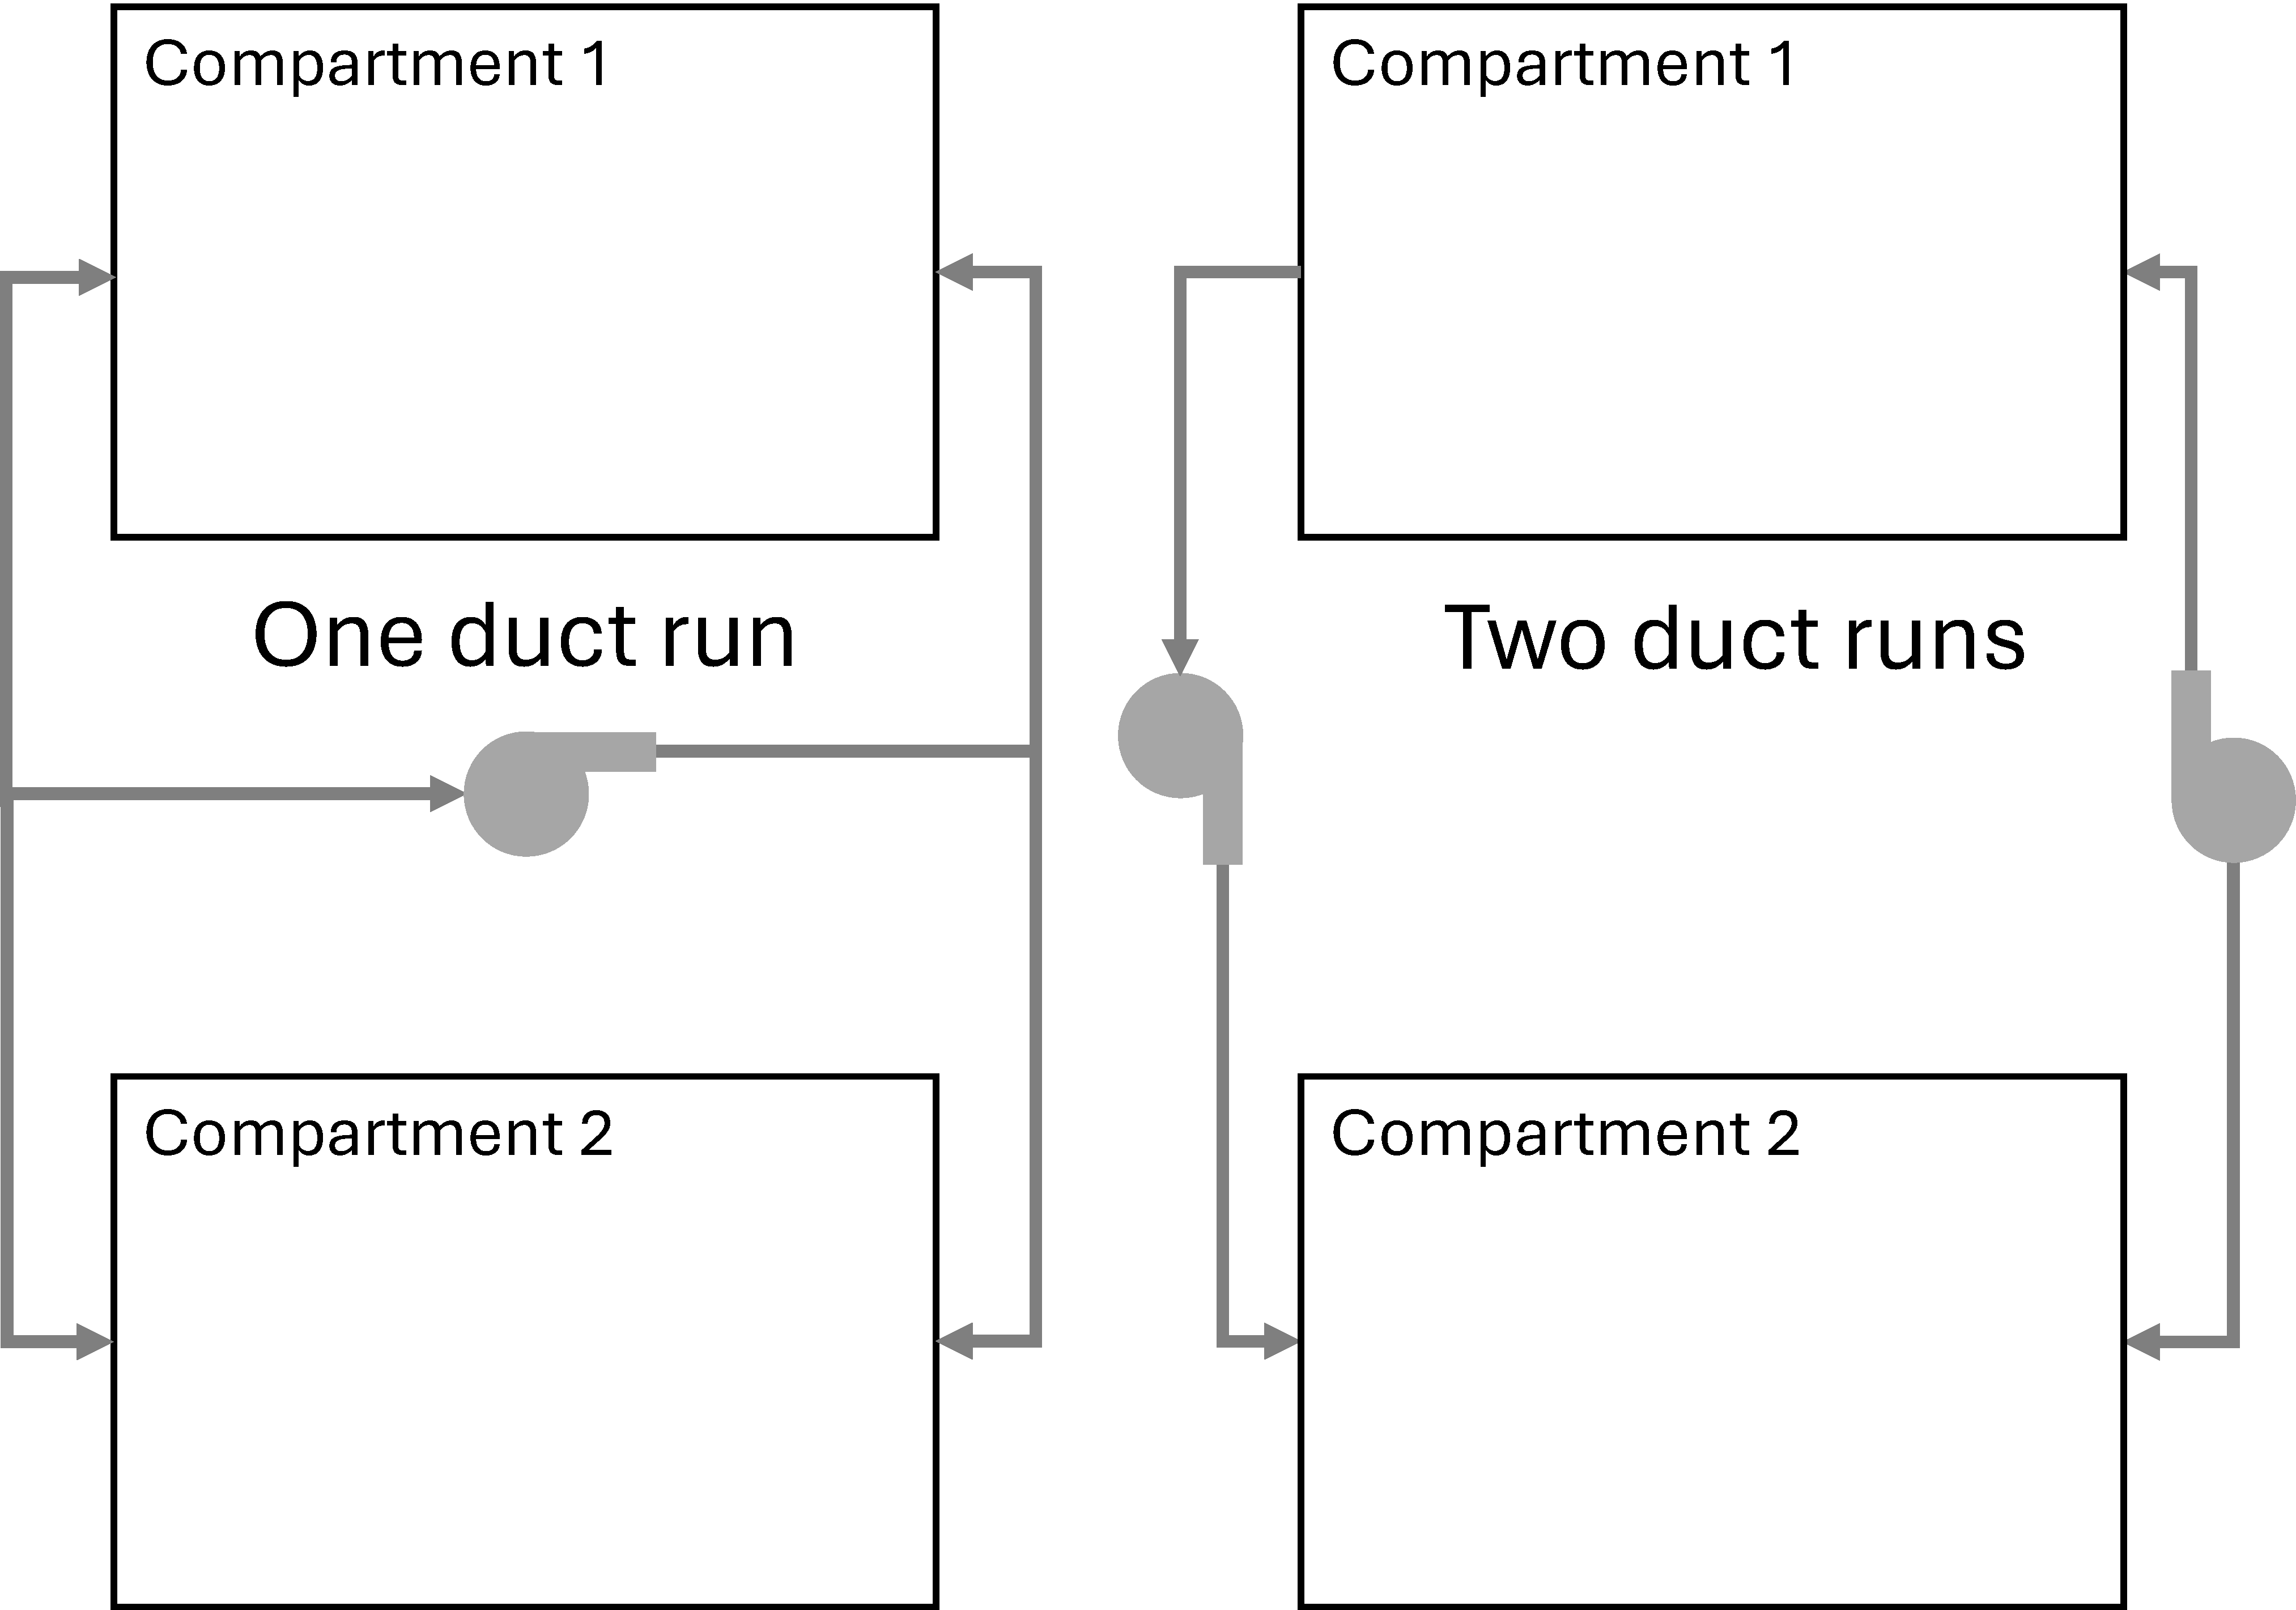
\includegraphics[width=\textwidth]{FIGURES/Compartment_duct_fan}}
      \caption[Illustration of determining duct runs]{\label{HVAC_ductrun} Illustration determining duct runs. Left side has a single duct run. Right side has two duct runs.}
   \end{center}
\end{figure}

\section{Duct Transport Delay}
\label{sec:duct_transport}

In its default mode of operation, the HVAC solver does not account for mass storage in ducts. That is over a time step any mass and energy entering a duct, leaves the duct. An optional submodel can be invoked to account for this transport delay. This submodel divides a duct into cells of equal length $\Delta x$ and solves a one dimensional advection equations for mass and energy transport in the duct~\cite{Ralph:3}. In the discretization, temperature, specific heat, species mass fractions, and density are stored at cell centers. The velocity in duct is taken as the value obtained from the solution of Eq.~(\ref{HVACmass}) through Eq.~(\ref{HVACmomentum}). An explicit Runge-Kutta method is used with a Godunov upwinding scheme. Diffusive transport is ignored as this is generally a minor effect in an HVAC system. The species mass and energy conservation equations for updating cell $c$ in duct $j$ from timestep $n$ to $n+1$ are:

\be (\rho \, Y_{\alpha})_c^{n+1}=  \rho_j \, u_j^n - \frac{\Delta t}{\Delta x} \, (\rho \, u)_j^n left(Y_{\alpha ,c}^n - Y_{\alpha ,c-1}^n ) \ee  
\be (\rho \, h)_c^{n+1}=  \rho_j \, u_j^n - \frac{\Delta t}{\Delta x} \, (\rho \, u)_j^n left(h_c^n - h_{c-1}^n ) \ee  

Updating duct conditions begins at the upwind duct node and marches over the duct length to the downwind duct node. Cell temperatures are extracted from the cell enthalpy $h_c$. This solution is done over groups of ducts that form a duct network basis. A duct network is a set of ducts and nodes that are interconnected via a flow path through HVAC components. The time step $\Delta t$ is taken as the minimum of the current simulation time step and the minimum value of $\frac{\Delta x_j}{2 u_j}$ over all ducts in the network. In the summation terms in Eq.~(\ref{HVACmass}) and Eq.~(\ref{HVACenergy}), the mass flow and enthalpy flow into a node from a discretized duct are obtained by integrating those flows using the values in the last cell over each time step taken.
